\chapter{Background on Text Generation}
\label{chap:background}
Automatic text generation has been a goal of computer science researchers since the early days of computing.
In recent years, template-based, grammar-based, and statistical approaches have given way to neural language models--neural networks trained to build representations of human language from millions or even billions of documents.
This chapter gives a brief overview of how modern text generation systems based on neural language models generate text.

\section{What is a Language Model?}
A language model is any model that assigns probabilities to sequences of words.
Given a sequence of words $w_1, \ldots, w_n$, a language model outputs the likelihood $P(w_1, \ldots, w_n)$ of this sequence.
An ideal language model would assign high likelihood to natural-sounding text, like the sentences in this paragraph, and  low likelihood to gibberish.
Most language models make the assumption that the likelihood of a word is dependent only on the words that precede it.
Thus, the chain rule applies:

\begin{align}
    \label{eq:lm_base}
    P(w_1, \ldots, w_n) = P(w_1) \times \ldots \times P(w_i | w_1, \ldots, w_{i-1}) \times \ldots \times P(w_n | w_1, \ldots, w_{n-1})
\end{align}
Before the transition to neural network-based models, the most common form of language model was a statistic language model called the $n$-gram model.
Instead of trying to estimate the probability of a word given all preceding words, $n$-gram models make the Markov assumption that the probability of a word is only dependent on a fixed $n$-1 preceding words\footnote{The $n$ in $n$-gram refers to the number of words used in the conditional probability distribution, and ``gram'' simply means ``word.''}.
For example, using a 3-gram model, we would approximate each factor in Equation \ref{eq:lm_base} as
\begin{align}
   P(w_i | w_1, \ldots, w_{i-1}) \approx P(w_i | w_{i-2}, w_{i-1})
\end{align}
An $n$-gram models can be constructed from a corpus of text by simply counting how many times each word in the text is preceded by each possible $n$-gram.
This is an advantage over grammar-based approaches to language modeling--such as statistical parsers--which require explicitly labeled training data, such as the Penn Tree Bank, in order to estimate probabilities.

There are several disadvantages to this $n$-gram based approach to language modelling.
First, $n$-gram models tend to be sparse.
If a particular <$n$-gram, word> pair never occurs in the corpus, then the model will assign it a probability of 0.
As a result, smoothing techniques are often employed to prevent plausible but novel word sequences from being assigned a probability of zero.
Second, the complexity of storing an $n$-gram language model grows exponentially with the choice of $n$.
In practice, most $n$-gram models used $n$ between 1 and 5, which is insufficient for modelling long-term dependencies and coherence.
Third, $n$-gram models do not adequately represent words which are not present in their training data.
Such words are typically replaced with a special out-of-vocabulary identifier.
Neural language models, described in the following sections, overcome many of these limitations.


\section{What is a Neural Language Model?}
\label{section:what_is_a_nlm}

Neural network-based language models replace the statistical models described in the previous section with a learned function (the neural network) whose output can be used to predict the likelihood of a word sequence.
In contrast to $n$-gram models, neural language models are capable of assigning non-zero probability to sequences never seen in their training corpora, and thus they can be used to model longer sequences.
State-of-the-art neural language models can model sequences in the thousands of words.

One of the key advances in neural language modeling was the transition from operating on sequences of discrete words to operating on sequences of continuous vector representations.
The sequence of words $w_1, \ldots, w_n$ is mapped to a sequence of embedding vectors $\by_1, \ldots, \by_n$.
In early work on neural language modeling, these vector representations were computed separately.
Algorithms such as word2vec \citep{mikolov2013word2vec} and GloVe \citep{pennington2014glove} were employed to construct embedding matrices where each row corresponded to a word in the vocabulary.
In today's neural language models, the embedding matrix is typically treated as part of the neural language model, initialized randomly than optimized along with the reset of the network.
Let $\mathbf{E}_\theta$ be a learned embedding matrix where each row correspond to the vector representation of one word in the vocabulary.

Typical neural language models emit $\hat{\by}_t$, a predicted embedding for the $t$th position in the sequence given the previous word embeddings in the sequence. This can be written as
\begin{align}
    \hat{\by}_t = f_\theta(\by_1, \ldots, \by_{t-1})
    \label{eq:lm_feq}
\end{align}

\noindent where $f_\theta$ is the neural network and $\by_1, \ldots, \by_{t-1}$ are the embeddings of the previous tokens in the sequence.

To produce a probability distribution for what the next word should be given the previous words, the predicted embedding $\hat{\by}_t$ is multiplied by the embedding matrix $\bE_\theta$ to produce a score for each word in the vocabulary.
Then a softmax transformation is used to normalize these scores into a probability distribution.
Let $Y_t$ be a random variable representing the vocabulary item predicted for the $t$th position. We then have:
\begin{align}
    \label{equation:vocab}
    P(Y_t=i | \by_1, \ldots, \by_{t-1}) = \frac{\exp(\bE\hat{\by}_t[i])}{\sum_j\exp(\bE\hat{\by}_t[j])}
\end{align}
where $i$ and $j$ are indexes into the vocabulary.

The learned weights $\theta$ are optimized using a log likelihood loss.
% In other words, the goal is produce an $\hat{\by}_t$ that is as close to the embedding of the true next word as possible.
More precisely, we can write the training loss for a sequence $\by_1, \ldots, \by_n$ as:

\begin{align}
\mathcal{L} &= -\sum_{t=1}^n \log P(Y_t=i^* | \mathbf{y}_{1:t-1}) \\
&= -\sum_{t=1}^n \log\frac{\exp(\mathbf{E}_\theta\hat{\mathbf{y}}_t[i^*])}{\sum_j\exp(\mathbf{E}\hat{\mathbf{y}}_t[j])} \label{eq:loss_2} \\
&= -\sum_{t=1}^n \mathbf{E}_\theta\hat{\mathbf{y}}_t[i^*] \label{eq:loss_3} \\
&= -\sum_{t=1}^n (\mathbf{E}_\theta f_\theta(\by_1, \ldots, \by_{t-1})[i^*]
\end{align}

In these equations, $i^*$ is the index of the groundtruth word at position $t$ in the sequence. 
By taking the dot product between the neural network's predicted embedding and the embedding of the true word at each position $t$ (Eq. \ref{eq:loss_3}), we get a score indicating how correct the neural network's prediction for this position is.
Training with an objective of maximizing the sum of these scores over every word position is equivalent to minimizing the negative log likelihood (or maximizing the likelihood) of the sequence.

In some language modelling applications, it is common to have an additional sequence on which the model is conditioned on in addition to the tokens of the target sequence.
This paradigm is known as an encoder-decoder or sequence-to-sequence model, and the formulation above is modified to
\begin{align}
    \hat{\by}_t = f_\theta(\by_1, \ldots, \by_{t-1}; \bx_1, \ldots, \bx_n)
    \label{eq:cond_lm_feq}
\end{align}
where $\bx_1, \ldots, \bx_n$ is the additional input sequence. 
The most popular application of encoder-decoder models is machine translation; for example, to convert some text from French to English, the language model predicts the next word of the English sequence given the entirety of the French sequence and the preceding words of the English sequence.

Most state-of-the-art neural language models use a variant of the Transformer architecture \cite{vaswani2017attention} as the neural network $f_\theta$.
Prior to the development of Transformers, recurrent neural architectures, typically based on Long Short Term Memory units \citep{hochreiter1997long}, were most commonly employed.
Transformers have several advantages over their recurrent predecessors, most notably that operations are parallelized across all tokens in the sequence.
This speeds up the computation time need for training immensely, and the computation time is no longer dependent on the length of the sequence.
Transformers are also much better than recurrent models at making connections between information that may be very far apart in the sequence.
Recurrent architectures keep track of a ``hidden state'' which gets updated for every position in the sequence.
A ramification of this sequential updating is that the final hidden state may no longer encode much information about the beginning of the sequence.
In contrast, Transformers use an ``attention mechanism'' that allows any position in the input sequence to easily ``attend'' to any other position.


\section{Encoding Text into a Vocabulary}

For simplicity, the previous sections refer to the input to a language model as a sequence of words, but in practice, neural language models use a variety of different techniques to construct vocabularies of varying granularities.
% divide text into a sequence of sub-word tokens, such as those produced by a Byte Pair Encoding (BPE) \citep{sennrich2016neural}.
% Typical BPE vocabularies range from 32k to 50k words.
% Only my work in Section \TODO{decide on section} uses an older word-level vocabulary.
There is no single solution for forming the base units of language (referred to for the remainder of this chapter as ``tokens''), and techniques vary significantly across languages.
In English, the simplest vocabularies are character-level--each letter of the alphabet and punctuation mark becomes a token.
Historically, word-level vocabularies, where each token corresponds to a word in the dictionary, were most common.
Word-level vocabularies can be created by splitting a string on whitespace and punctuation.
Since in most languages, the number of fully inflected words is enormous, in practice only the most common tens or hundreds of thousands of words are included in the vocabulary, and all other words are replaced with an out-of-vocabulary (OOV) token.

In recent years, subword vocabularies, which eliminate the OOV problem, have become standard in neural language modeling.
Subword vocabularies are formed by choosing a budget (the desired size of the vocabulary), then running an algorithm that joins letters together into larger units, such that the most common character sequences end up as tokens in the vocabulary.
While common words such as ``cat'' or ``dog'' end up as single tokens in the vocabulary, uncommon words such as hippopotamus end up bring broken into multiple tokens.
Several greedy algorithms have been proposed to approximate optimally breaking up a text corpus into subwords, but byte-pair encoding (BPE) is currently the most popular \citep{sennrich2016neural}.
Typical subword vocabulary sizes are between 32,000 and 50,000 tokens.
Table \ref{tab:tokenization} shows a sentence under a few different tokenization schemes.

\begin{table}[h]
    \centering
    \caption{Examples of the string ``A hippopotamus ate my homework." tokenized using three different vocabularies. With the subword tokenizer, the rare word ``hippopotamus" gets broken up into multiple tokens. For word-level tokenizers, if the word ``hippopotamus'' occurs very infrequently in the corpus used to build the vocabulary (or perhaps the writer of the sentenced misspelled it), it would typically get replaced with an out-of-vocabulary token (row 4).}
    \label{tab:tokenization}
    \begin{tabular}{l|p{5in}}
        Vocab Type & Example \\
        \hline
        character-level & \texttt{['A', ' ', 'h', 'i', 'p', 'p', 'o', 'p', 'o', 't', 'a', 'm', 'u', 's',' ', 'a', 't', 'e', ' ', 'm', 'y', ' ', 'h', 'o', 'm', 'e', 'w', 'o', 'r', 'k', '.']}\\
        subword-level & \texttt{['A', 'hip', '\#\#pop', '\#\#ota', '\#\#mus', 'ate', 'my', 'homework', '.']}\\
        word-level & \texttt{['A', 'hippopotamus', 'ate', 'my', 'homework', '.']}\\
        word-level & \texttt{['A', '[UNK]', 'ate', 'my', 'homework', '.']}\\
    \end{tabular}
\end{table}

For all of the types of vocabularies discussed, a decision must be made on whether to convert strings to lowercase before vocabulary creation.
Removing case allows for a more compact vocabulary, but it also removes potentially useful information about the location of proper nouns.

Subword vocabularies were designed to be a compromise between the advantages and disadvantages of word-level and character-level vocabularies.
Character-level vocabularies are usually very small, no more than a couple hundred tokens.
However, the vocabulary can cover nearly every possible string a person could write.
Word-level vocabularies cannot feasibly contain the hundreds-of-thousands of words present in English text.
Realistically, only the most common words are kept, and less common ones are replaced with a special \texttt{UNK} token.
When text is tokenized with character-level vocabularies, the resulting sequences are very long, while word-level tokenization yields shorter sequences since there is just one token per word.
Lastly, word-level representations learned by a neural net tend to be more meaningful than character-level representations since a word has semantics associated with it that are common across uses.
Subword vocabularies adopt the best of both worlds, using word-level tokens for common words but falling back to subword, or in the worst case, character-level, tokenization for uncommon words.
This approach eliminates the need for an out-of-vocabulary token and results in tokenized sequence lengths which are somewhere between the two strategies.


\section{Generating Text with a Language Model}
\label{section:background_gen}

Neural language models in themselves are capable of generating text.
As described in the previous sections, most language models provide a probability distribution for what the next token in the sequence \textit{could} be, given the previous tokens.
To perform generation, an algorithm is needed that chooses which words to output given the model's predicted probability distributions.
We refer to this family of algorithms as \textbf{decoding methods} because they ``decode'' a sequence of discrete words from the model's predictions.
At each step of decoding, the decoding algorithm performs a forward pass on the neural network using the existing prompt text as input, selects a next token based on the neural network's predictions, adds this token to the prompt, and repeats until the desired number of tokens have been generated.

\subsection{Greedy Approaches}
The simplest strategies for generating text from a language model involve greedily choosing a token at each step.
The easiest way to do this is to take the $\arg \max$ of the distribution, repeatedly picking the token with the highest probability according to the model.
This approach is simple but only allows a single generation to be produced for any given prompt.
Alternatively, one can randomly sample from the vocabulary, where each vocabulary item has a chance of being picked that is proportional to the probability predicted for it by the language model.
This method allows for many different sequences to be generated from the same prompt.
However, in practice, this strategy results in text that is perceived as nonsensical and otherwise low-quality.
This is because the probability distributions returned by neural language models tend to be very long tailed, and the chance of sampling a rare/unusual word from this long tail is quite high. For example, if we sample from the full distribution words that could follow \texttt{The dog ate my}, with low probability we might sample \texttt{brains}, even though \texttt{homework} is much more probable.

Several strategies have been proposed to improve random sampling techniques by reducing the entropy of the distribution before sampling.
Introducing a temperature parameter $\tau$ into the softmax computation allows us to smoothly shift probability mass from low-scoring items in the vocabulary to high-scoring ones.
\begin{align}
    \label{equation:softmax_with_temp}
    P(Y_t=i | \by_1, \ldots, \by_{t-1}) = \frac{\exp(\bE\hat{\by}_t[i]/\tau)}{\sum_j\exp(\bE\hat{\by}_t[j]/\tau)}
\end{align}
Alternatively, one can introduce sparsity intro the distribution by deliberately zeroing out low-likelihood vocabulary items.
Top-$k$ random sampling accomplishes this by restricting sampling to only the $k$ most likely tokens at each step.
Nucleus sampling, also referred to as top-$p$ random sampling, accomplishes this by restricting sampling at timestep $t$ to the $k_t$ most likely tokens, where $k_t$ is selected such that these tokens cover no more than $p$\% of the probability mass.
For all three of these techniques there is a parameter ($\tau$, $k$, or $p$) which controls the amount of randomness we want to permit in the generation.
Choosing a low value for these parameters results in an increasingly peaky distribution, which, at its extreme, is the same as taking the $\arg \max$. 
Choosing a high value for these parameters results in the distribution that looks closer to the original scores produced by the model.
% Figure \TODO{Add figure showing some probability distributions.} shows how these different strategies affect the shape of the distribution.

\subsection{Search-Based Approaches}
Before the transition to Transformer-based architectures (Section \ref{section:what_is_a_nlm}), the standard convention for generation was to try to generate the most likely overall sequence from the language model.
This approach made a lot of sense for the predominant use case of machine translation, where generating one correct translation was considered more important than generating several diverse translations.
Since computing the overall most likely output sequence is intractable, early work in neural machine translation found that beam search was an effective strategy to heuristically sample sufficiently likely sequences from these probabilistic models \cite{sutskever2014sequence}.

Algorithm \ref{alg:beam-search-inference} gives an overview of the beam search algorithm. 
``SOS'' is a start-of-sequence token and ``EOS'' is an end-of-sequence token.

\begin{algorithm}
\caption{Beam Search Inference}
\label{alg:beam-search-inference}

\begin{algorithmic}[1]
\Procedure{Beam Search}{}
\State $B \gets \{SOS\}$
\State $k \gets $ BeamWidth
\State $out \gets k$-best output list
\While{$|out| < k$}
    \State $front \gets \text{remove all nodes from} B$
    \For{$w \in front$}
    \State $succ \gets w$'s $k$-best successors
    \For{$s \in succ$}
    \If{$s == EOS$}
        \State $out \gets out \cup \{s\}$
    \Else
        \State $B \gets B \cup \{s\}$
    \EndIf
    \EndFor
    \EndFor
    \State Sort $B$
    \If{$|B| > k$}
        \State Prune $B$ to $k$-best successors
    \EndIf
\EndWhile

\Return out
\EndProcedure
\end{algorithmic}
\end{algorithm}

As neural language models came to be applied increasingly to open-ended tasks, such as chatbot dialog or story generation, beam search was found to be ill-suited to generating a set of \textit{diverse} candidate sequences
Since beam search only explores a limited portion of the overall search space, it tends to yield multiple variants of the same high-likelihood sequence.
The outputted sequences often only differ in punctuation or minor morphological changes \cite{li2016mutual}.  
To try and solve this problem, many researchers proposed modification to beam search to encourage it to produce more diverse sets of candidate generations.
We summarize several of these here:

\begin{itemize} 
\item \textbf{Noisy Parallel Approximate Decoding.}\quad
Introduced by \citet{cho2016noisy}, NPAD is a technique than can be applied to any decoding setting.
The main idea is that diversity can be achieved more naturally by taking advantage of the continuous manifold on which neural nets embed language.
Instead of encouraging diversity by manipulating the probabilities outputted from the model, diverse outputs are instead produced by adding small amounts of noise to the hidden state of the decoder at each step.
The noise is randomly sampled from a normal distribution. The variance is gradually annealed from a starting $\sigma_0$ to 0 as decoding progresses (that is $\sigma_t = \frac{\sigma_0}{t}$) under the reasoning that uncertainty is greatest at the beginning of decoding.
NPAD can be used in conjunction with any decoding strategy, though the paper in which it was introduced primarily showed its performance in conjunction with beam search.

\item \textbf{Top-$g$ Capping.}\quad
In beam search, it is often the case that one hypothesis $h$ is assigned a much higher probability than all other hypotheses, causing all hypotheses in the next step to have $h$ as their parent. Li et al. \citep{li2016mutual, li2016simple} proposed adding an additional constraint to standard beam search to encourage the model to choose options from diverse candidates.
At each step $t$, current hypotheses are grouped according to the parental hypothesis they come from.
After grouping candidates, only the top $g$ from each grouping are considered. The resulting $b \times g$ candidates are ranked, and the top $b$ are selected as hypotheses for the next beam step.

\item \textbf{Hamming Diversity Reward.}\quad
\citet{vijayakumar2016diverse} proposed adding an additional diversity-promoting term, $\theta$, to the sequence log-likelihoods before the reranking step of beam search.
This term measures how different a candidate hypothesis $c^{(i)}_{\leq t}$ is from the partial hypotheses selected in the previous step. Let $\mathcal{H}_{t-1} = \{c^{(1)}_{\leq t-1}$, \ldots $c^{(b)}_{\leq t-1}\}$ be these partial hypotheses.
Then the beam search scoring function for the $i$th candidate at timestep $t$ becomes:
\begin{align*}
    \text{score}(c^{(i)}_{\leq t}) = \sum_{j=1}^t \big(\log P(c^{(i)}_j | c^{(i)}_{<j}, \textbf{x})\big) \\+ \lambda\theta(c^{(i)}_{\leq t}, \mathcal{H}_{t-1})
\end{align*}
where $\lambda$ is a tunable hyperparameter. \citet{vijayakumar2016diverse} try a variety of definitions for $\theta$, including embedding diversity and $n$-gram diversity, but they find that Hamming distance, the number of tokens in the candidate sequence which exist in the previously selected partial hypotheses, is most effective. 

\item \textbf{Iterative Beam Search.}\quad
In an attempt to improve the size of the search space explored without sacrificing runtime, Kulikov et al. \citep{kulikov2018importance} propose an iterative beam search method.
Beam search is run many times, where the states explored by subsequent beam searches are restricted based on the intermediate states explored by previous iterations.
Formally, they define the set of all partial hypotheses for beam search instance $i$ at time step $t$ as $\mathcal{H}_t^{(i)}$. From here, the search space explored by beam search instance $i$ can be expressed as $S_i = \cup_{t=1}^T \mathcal{H}_t^{(i)}$.
The $i$th beam search is prevented from generating any partial hypothesis that has previously been generated, that is, any hypothesis found in $S_{<i} = \cup_{i^{\prime}=0}^{i-1}S_{i^{\prime}}$.

\item \textbf{Clustered Beam Search.}\quad
\citet{tam2019clustered} proposed a clustering-based beam search method to help condense and remove meaningless responses from chatbots.
Specifically, at each decoding step $t$, this method initially considers the top $2*b$ candidates. From there, each candidate sequence is embedded\footnote{We follow \citet{tam2019clustered} and used averaged GloVe word embeddings \cite{pennington2014glove}.}, and the embeddings are clustered into $c$ clusters using $K$-means. Finally, we take the top $\frac{b}{c}$ candidates from each cluster. Note that in the case any clusters have size less than $\frac{b}{c}$, we then include the highest-ranked candidates not found after clustering.

\subsection{Generation Diversity}
For many tasks, especially open-ended ones like story generation or chitchat dialog, it is important for generated text to be ``diverse.''
The term ``diversity'' has been used in the language model literature to refer to a diverse set of properties.
Some use it as a synonym for sentence interestingness or unlikeliness \citep{tatsunori2019unifying}.
Others consider diversity a measure of how different two or more sentences are from each other \citep{vijayakumar2016diverse,gimpel2013systematic}.
In some framings, diversity is measured across a set of generations coming from the same prompt.
Given a particular prompt or input, the goal is to measure the breadth of possible generations the model will produce \citep{mayhew2020simultaneous}.
Diversity can also be measured at a corpus-level: given all the sentences generated by the model for all prompts, what is the overall lexical diversity?

In my research, I use three definitions of diversity.
First, when performing conditional generation, I define diversity as the ability of a generative method to create a set of possible outputs that are each valid given a particular input but vary as widely as possible in terms of word choice, topic, and meaning.
Second, when performing unconditioned generation using decoder-only language models, I instead consider corpus-level diversity across all the model's generations--how much lexical variety is there over all the text the model generated?
Finally, in some of my work, I ask human raters to evaluate generation interestingness, which is a measure of human-perceived diversity.


\subsection{Generation Quality}
For all generation tasks, it is important for the output text to be high quality, though this property can also be difficult to define.
In some downstream applications, ``quality'' can be evaluated directly
by asking human raters questions like "How good is this text?"
(though question phrasings and explanations of what it means to be ``good'' vary widely across the literature \citep{van2019best}).
In others, it can be quantified as how many times a user interacts with the generative system (for example, the number of conversation turns with a dialog agent) before losing interest.

To some extent, quality can also be measured automatically.
In tasks with a clear goal, like machine translation or summarization, one can compare the generation against a gold standard.
Quality is strongly associated with fluency: it is generally true that the lower perplexity a language model assigns some text, the more fluent the text is, and thus the higher quality.
However, my collaborators and I show that this relationship between quality and perplexity breaks down for extremely high-likelihood generated text \citep{zhang2021trading}.

In some of my research, we evaluate quality by asking humans to assess generations in terms of their fluency, adequacy, and interestingness.
In Chapter \ref{chap:decoding}, we propose a novel method for assessing generation quality based on the premise that humans (or a trained discriminator) ought to have a hard time distinguishing between real human-written text and model outputs when the model produces text that is high-quality.

\subsection{The Diversity-Quality Tradeoff}
The goal of generating high-quality text is often at odds with the goal of generating diverse text.
In experiments conducted with Reno Kriz \citep{ippolito2019comparison}, I found that none of the diversity-promoting search methods accomplished their stated goal of improving diversity without significant penalty to generation quality.
In our experiments, we compared all of the diverse beam search methods described above with standard beam search as well as several settings of random sampling with temperature.
On an open-ended dialog task, we showed that human-judged generation quality was inversely correlated with three measures of diversity (Figure \ref{fig:correlations}).

For each utterance in the dialog task validation set, we generate 10 candidate outputs using each decoding method.
To measure the diversity across the generated candidate sequences for a given input utterance, we compute \textbf{Dist-k}, the total number of distinct k-grams divided by the total number of produced tokens in all of the candidate responses for a prompt \citep{li2016diversity}. 
We use $k$=2.
A limitation of Dist-$k$ is that all $k$-grams that appear at least once are weighted the same, ignoring the fact that infrequent $k$-grams contribute more to diversity than frequent ones. 
Therefore, we also report Zhang et al.'s \citep{zhang2018generating} proposed entropy metric, \textbf{Ent-k}, defined as:
 \begin{align*}
 \textit{Ent-k} = \frac{-1} {\sum_{w \in S}F(w)} \sum_{w \in S} F(w) \log \frac{F(w)} {\sum_{w' \in S} F(w')}
 \end{align*}
 where $S$ is the set of all $k$-grams that appear in candidate responses for an example, and $F(w)$ denotes the frequency of $w$ in the candidate responses.
Finally, we report \textbf{perplexity}, averaged over \textit{all} the top 10 outputs for each example.

\begin{figure}[ht]
    \centering
    \begin{subfigure}[l]{5cm}
        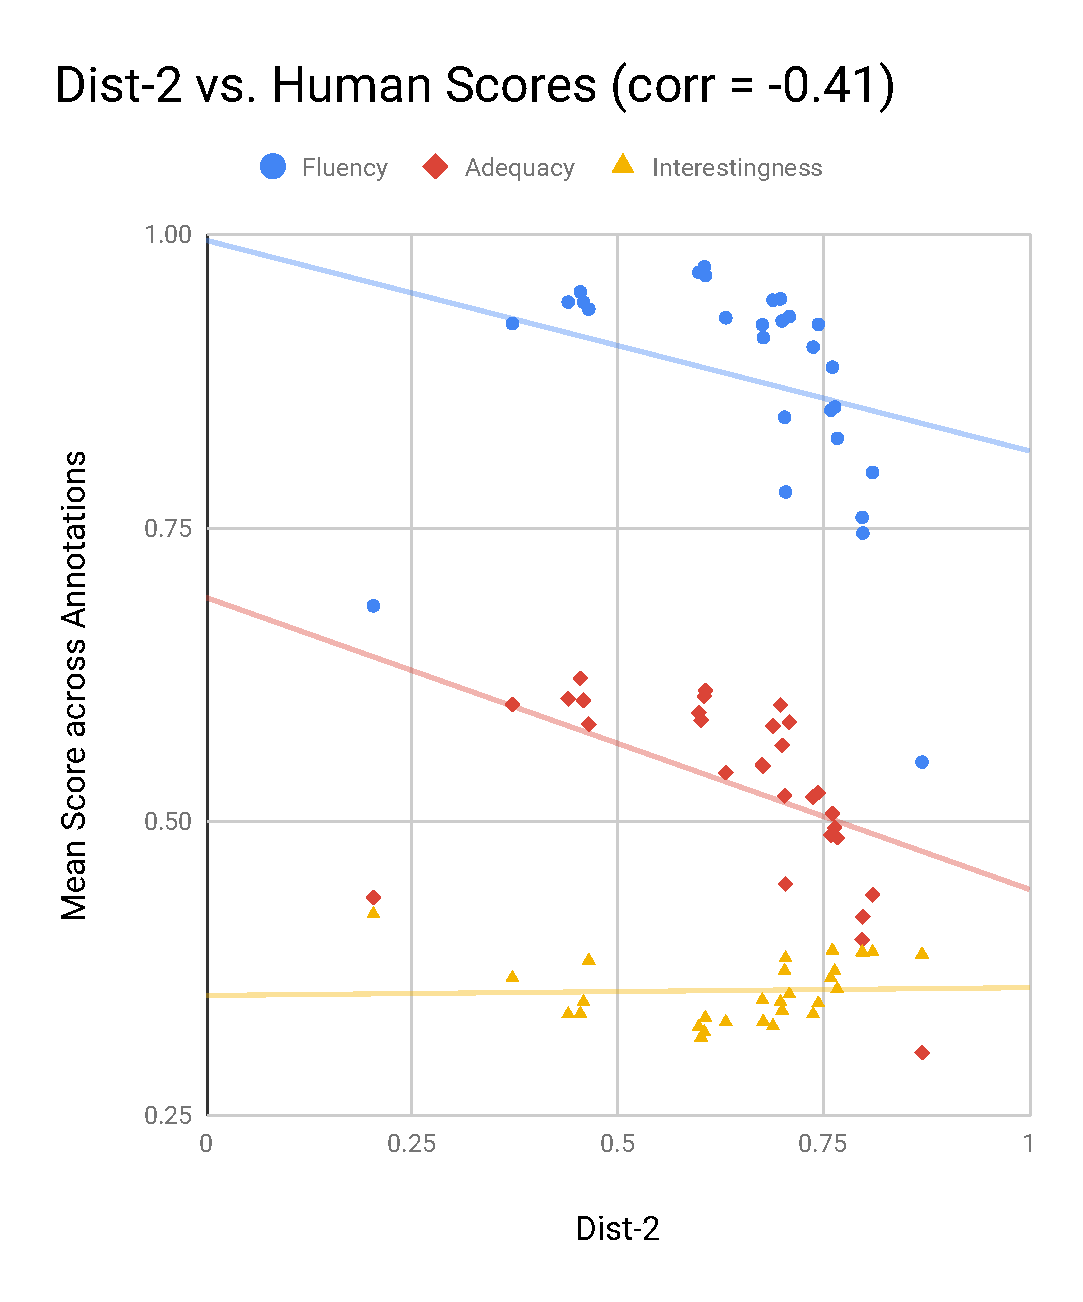
\includegraphics[width=5cm]{figures/dist2_vs_human.pdf}
    \end{subfigure}
    \begin{subfigure}[l]{5cm}
        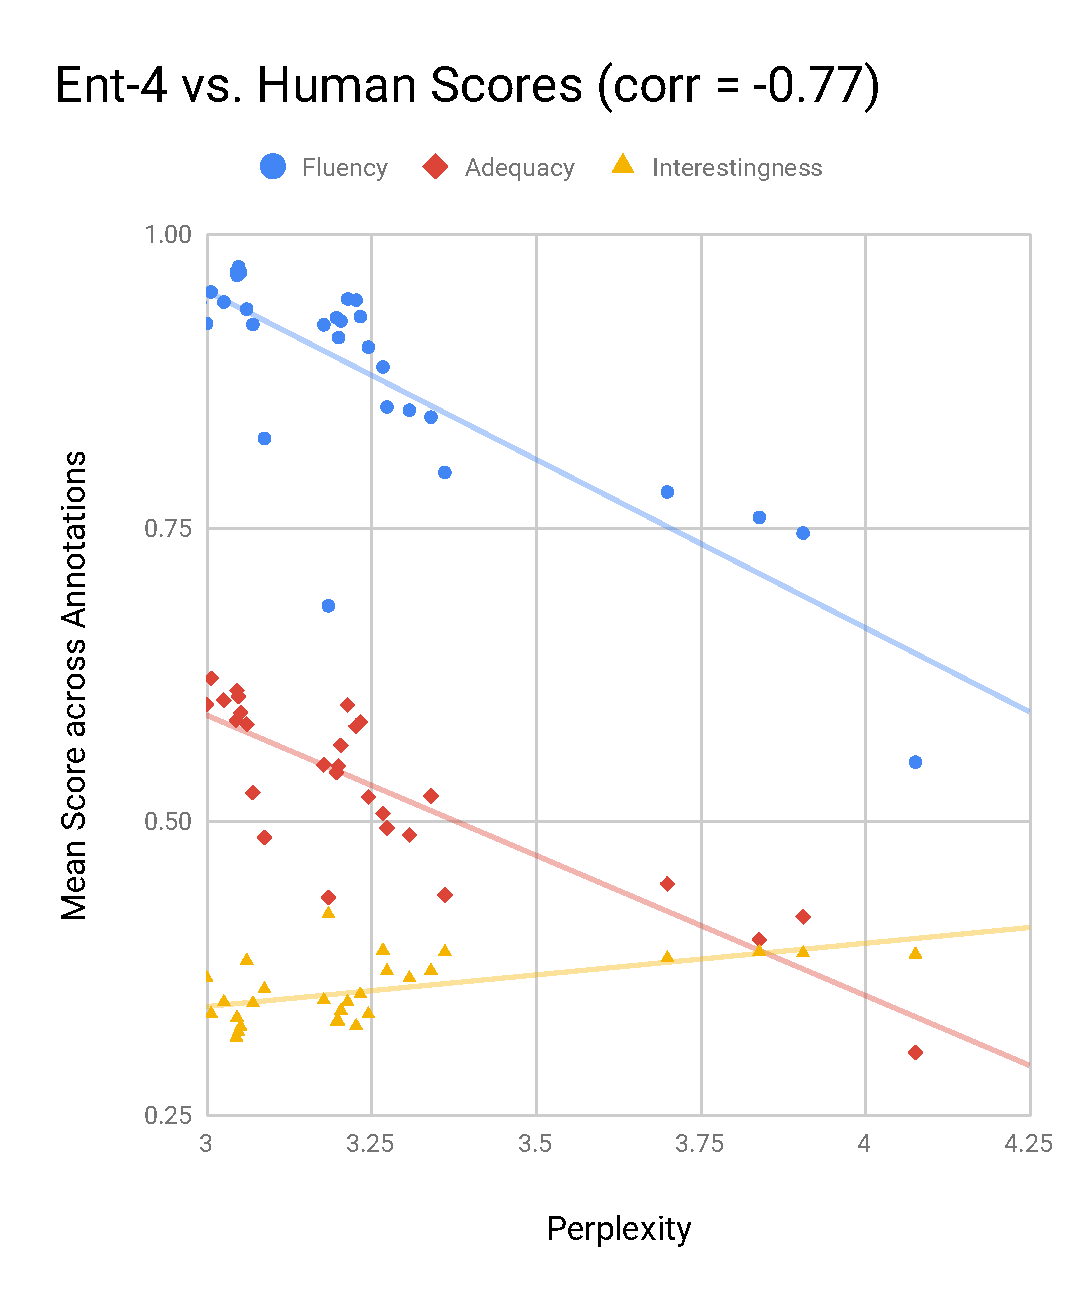
\includegraphics[width=5cm]{figures/ent4_vs_human.pdf}
    \end{subfigure}
    \begin{subfigure}[l]{5cm}
        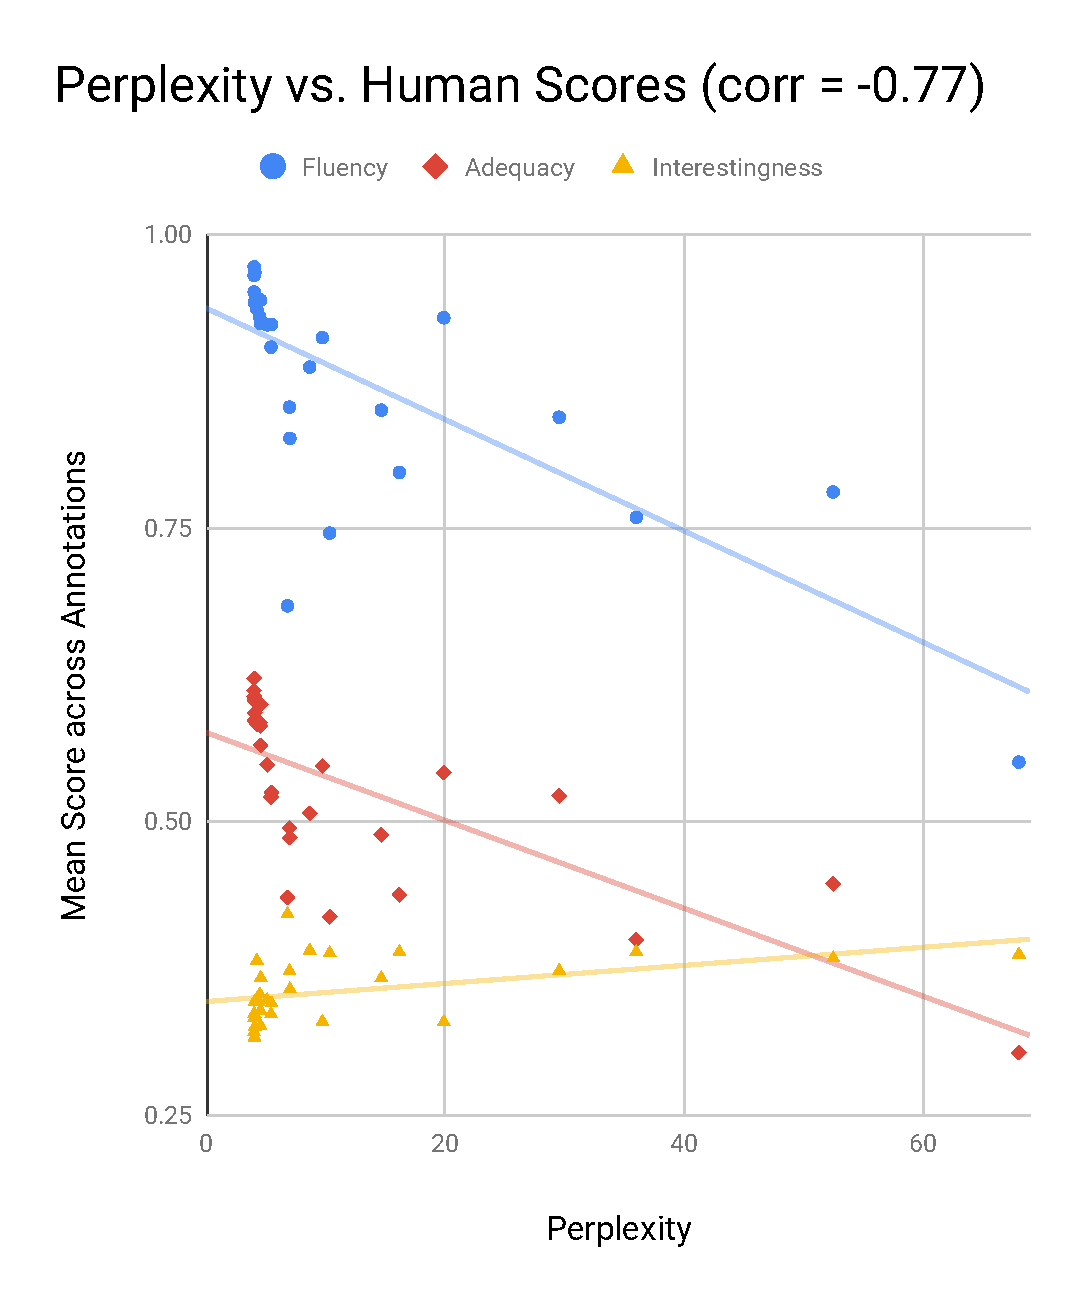
\includegraphics[width=5cm]{figures/perplexity_vs_human.pdf}
    \end{subfigure}
    \caption{Each point corresponds to the outputs from one decoding strategy. 
     The x-axes give the dist-2, ent-4, and perplexity scores of the generated text.
     The y-axes give the human-judged fluency, coherence, and interestingness of the outputs on a scale from 0 to 1.
     The Pearson Correlation coefficients between each statistic and the average of fluency, coherence, and interestingness are shown in parentheses.}
    \label{fig:correlations}
\end{figure}

For all three diversity measures, we see that the decoding strategies which produce the most diverse text also produce the least fluent and least adequate responses to the input utterances.
For example, given the prompt ``\texttt{Look, nobody knows we did it.}'' random sampling generates the candidate responses ``\texttt{We didn’t have a plan I engineered a policy.}'' and ``\texttt{Same time you pick us up at six and get we.}''
These are interesting but don't make much sense.
In contrast, beam search generates ``\texttt{I don’t know what to say},'' which is neither interesting (as evaluated by human raters) nor diverse (many generated responses started with \texttt{I don't know}).
However, it is a reasonable response to the prompt.

One important consequence of the diversity-quality tradeoff is how detectable the generated text is to humans and automatic discriminators.
The relationship between detectability and the lexical diversity of model generations is described in detail in Chapter \ref{section:detection}.

\section{Language Generation Tasks in This Dissertation}
My dissertation touches upon several tasks in language generation.
A brief summary of each task, as well as the means by which performance is evaluated, is provided here:

\paragraph{Continuation}
An NLG system is asked to generate a continuation for a prompt. It is then evaluated on how closely the generated continuation matches the true continuation. Automatic evaluation can either be performed using word overlap metrics such as BLEU \citep{papineni2001bleu}, or by measuring fluency (computing the perplexity of a model on the generated continuation).
Human evaluation usually involves showing a rater the prompt and generation and asking them to make some decision about it.
In Chapter \ref{section:detection}, the decision is to try and distinguish whether or not the presented text was machine-generated or not.

\paragraph{Fill-in-the-blank}
The fill-in-the-blank or infilling task is similar to continuation, except that the system also has access to the text which should occur \textit{after} the generation.
Evaluation is similar to evaluating continuation.
Chapter \ref{section:fitb} describes this task in detail.

\paragraph{Chitchat Dialog}
Chitchat dialog is the task of predicting the next utterance in a conversation given the previous turns.
As described in the previous section, we evaluate how choice of decoding strategy impacts the ability of an NLG system to produce an utterance that is both high quality and diverse.
In addition to conducting automatic evaluation with BLEU and perplexity, human evaluation can be performed by asking raters to evaluate each generated utterance in terms of fluency, adequacy, and interestingness.

\paragraph{Textual Style Transfer and Rewriting}
Textual style transfer is the task of taking an input passage of text and a desired style and rewriting the input text to reflect that style.
Typical tasks include sentiment transfer (for example, rewrite a negative restaurant review to have positive sentiment) and formality transfer (rewrite informal language to be formal).
In my work, I am broadly interested in the task of rewriting input text to fulfill a user-specified writing objective.
These rewriting tasks are a superset of style transfer; for example a user may ask for text to be ``rewritten to include the word 
\textit{balloon}'' or to ``have a cliffhanger at the end.''
Such rewriting could change both the content and the style.
We evaluate rewriting using automatic metrics, such as measuring how often an automatic classifier identifies the rewritten task as having fulfilled the rewriting goal.
We can also use metrics like BLEU score to compare against both the input sentence and a human-written groundtruth, although word-overlap metrics break down when the writing text is more open-ended or transformational.
Finally, human raters can be used to assess quality of the rewrite.

\paragraph{Story Ideation and Brainstorming}
For many writers, the process of writing is collaborative.
They may use an ideation tool such as a deck of trigger cards to come up with initial ideas, or they may share their in-progress draft with readers to get feedback.
One of the goals of my research is to be able to use neural language models to provide an alternative collaboration source for creative writers.
This includes a suite of user-defined tasks centered around allowing writers to make requests such as ``what should happen next in my story?'' or ``help me write a description of the old man introduced in the first sentence.''
Because the goals here are so broad, evaluation is best done holistically--by conducting user studies to evaluate whether NLG outputs are useful to human writers in their writing goals.

\section{Controllability and Task-Specific Generation}

In the early days of neural language modeling, it was common to train a separate neural language model for each NLG task of interest.
For example, if one wanted a system capable of producing chatbot dialog, one would train their neural language model on a dialog dataset (or close approximate) such as OpenSubtitles \citep{vinyals2015neural}.
If one wanted a system able to perform text summarization, one would likewise train a model from scratch on a dataset such as the CNN/Daily Mail corpus \cite{nallapati2016abstractive,DBLP:journals/corr/SeeLM17}.
At the time, the neural networks being used for these sorts of tasks were relatively small, and training and maintaining one model per task, was mostly feasible.

In 2018, Howard and Ruder \citep{howard2018universal} and Radford et al. \citep{radford2018improving} concurrently proposed the idea of pre-training a single universal task-agnostic language model.
To accomplish any specific language task of interest, that model could subsequently be trained for extra steps on the training data of the desired task, a process known as \textit{finetuning}.
The idea of finetuning a more general model for a specific task took off in computer vision when researchers showed that a convolutional neural network pre-trained on the ImageNet task of classifying the contents of images could be finetuned for tasks ranging from semantic image segmentation \citep{orsic2019defense} to cancer detection \citep{cadrin2022moving}.

General-purpose language models intended for generation tasks tend to be pre-trained on massive datasets scraped from the internet (Table \ref{tab:dataset_list}).
It is common to use both decoder-only models trained only to predict the next token given the previous ones \citep{radford2019language}, as well as encoder-decoder architectures trained with a de-noising loss, in which the input is a corrupted version of the text, and the task is to recover the uncorrupted text \citep{raffel2019exploring,lewis2020bart}.
Table \ref{tab:common_pretrained_models} gives examples of several pre-training objectives that have been employed by popularly-used pre-trained models.
Each of these models has been finetuned for a large diversity of downstream tasks.

\begin{table*}
  \centering
  \small
  \caption{A survey of datasets which have been used to train large general-purpose neural language models.}
  \label{tab:dataset_list}%
    \begin{tabular}{l|l|l|l|l}
    \toprule
    \textbf{Dataset} & \multicolumn{1}{l}{\textbf{Size}} & \multicolumn{1}{l}{\textbf{Public?}} & \textbf{Language} & \multicolumn{1}{l}{\textbf{Models trained on it}} \\
    \hline
    C4 \citep{raffel2019exploring}   &  365M examples,      & {Yes} & Most English & {T5} \\
    mC4 \citep{xue2020mt5}   &  8.5B examples  & {Yes} & 101 languages & {mT5} \\
    The Pile \citep{gao2020pile} & 825 GiB & {Yes} & Mostly English & {GPT-Neo, Megatron-Turing} \\
    RealNews \citep{zellers2019defending} &   120GB    & {Yes} &   English & GROVER    \\
    PanGu-$\alpha$ train set \citep{zeng2021pangualpha} & {1.1TB} & {No} & Chinese & {PanGu-$\alpha$} \\
    WebText \citep{radford2019language} &  40 GiB & {No} & Mostly English &  {GPT-2} \\
    GPT-3 train set \citep{brown2020language} & {500B tokens} & {No} & Mostly English & {GPT-3} \\
    \bottomrule
    \end{tabular}%
\end{table*}%


\begin{table}
    \centering
    \small
    \caption{Examples of pre-training objectives used in popular general-purpose models.
    In these examples, the original training sequence is ``\texttt{The hippopotamus ate my homework. It made me very mad.}''}
    \label{tab:common_pretrained_models}
	\begin{tabular}{l|p{2in}|p{2in}}
        \toprule 
        \textbf{Model} & \textbf{Input} & \textbf{Objective} \\
        \hline
        BERT \citep{devlin2018bert} & \texttt{[cls] The hippopotamus [mask] my homework. [SEP] It made me very [mask] . [sep]} &  Predict tokens for [mask] positions and predict whether the two sentences are in the correct order.\\
	\midrule
        T5 \citep{raffel2019exploring} & \texttt{The hippopotamus [x] made me [y] mad.} & Predict missing sequences.  \\
	\midrule
        BART & \texttt{It \_ me very mad. The hippopotamus my \_.} &  Predict the original uncorrupted sequence from a version that has been noised (token masking/deletion, text infilling, document rotation, sentence shuffling). \\
	\midrule
        GPT \citep{radford2019language,brown2020language} & \texttt{The hippopotamus ate} & Predict the next token given the previous tokens.\\
        \bottomrule
    \end{tabular}
\end{table}

Finetuning such models has yielded immense success in tasks across the field of natural language processing.
Chapter \ref{section:fitb} focuses on the feasibility of finetuning for the fill-in-the-blank task.
There are, however, several limitations to the paradigm of pre-training followed by finetuning.
As state-of-the-art neural language models increase in number of parameters, the computational expense of finetuning is becoming increasingly prohibitive.
Furthermore, the need to store (potentially in GPU memory) one set of model weights per task makes it very difficult to build downstream applications which need to perform several different tasks.
In addition, finetuning only works when there is enough on which data to fine-tune.
Overfitting is a significant challenge when training or finetuning in low-resource settings, where there may only be a handful of training examples.

For these reasons, various approaches have been proposed for replacing the finetuning step with methods which require either no or minimal weight training.
Brown et al. \citep{brown2020language} introduce the technique of \textit{few-shot prompting}.
By constructing a textual prompt which contains several examplars of the goal task, a general-purpose language model can be made to perform the task.
Lester et al. \citep{lester2021power} introduce \textit{prompt tuning} as an improvement over few-shot prompting that trains a small neural network to produce an optimal prompt in embedding-space for the goal task.

In this dissertation, I explore both finetuning and few-shot prompting.
Chapter \ref{section:style_transfer} uses prompting techniques for the task of textual style transfer, while Chapter \ref{section:wordcraft} shows how these techniques may be used for a variety of story editing operations.
Chapter \ref{section:fitb} focuses on fill in the blank, a task where finetuning outperforms other more training-efficient methods.
